%% Chickenizer CSC 343 term paper (single column, 11pt, numeric citations).
\documentclass[11pt]{article}
\usepackage[margin=1in]{geometry}
\usepackage{amsmath,amssymb}
\usepackage{graphicx}
\usepackage{booktabs}
\usepackage{caption}
\usepackage[hyphens]{url}
\usepackage{xurl}
\usepackage[numbers,sort&compress]{natbib}
\usepackage[hidelinks]{hyperref}
\setlength{\emergencystretch}{3em}
\newcommand{\filepath}[1]{\path{#1}}

\title{Chickenizer: Integrating Logic, Equilibrium Analysis, Simulation, and Learning for Strategic Play in Chicken}
\author{Greyson Henry\\Will Zoeller}
\date{April 22, 2026}

\begin{document}
\maketitle
{\small
\noindent\textbf{Repository:} \url{https://github.com/Alvin-Furman-CS-Classroom/project-2-ai-system-chickenizer}\\
\textbf{Demo:} If you run the Streamlit app locally, use \texttt{python -m streamlit run .src/ui/streamlit\_app.py} from the repo root, then open \url{http://127.0.0.1:8501} (default port). Replace the GitHub URL with your real remote; replace the demo line with a hosted URL or recording link if you submit one.
\par\vspace{0.6em}}
\pagestyle{plain}

\begin{abstract}
Chicken is a simple model of escalation: if both players push, both can lose badly; if one pushes and the other yields, the pusher often gains at the other's expense. Chickenizer is a Python system for a turn-based variant with richer state (health, resilience, and preference weights). It combines three views of the same game: strategy rules encoded as logic and checked with SymPy~\cite{sympy}; a simulation engine that plays strategies round by round; and a $2\times 2$ normal form built from one-shot counterfactuals, with pure and mixed Nash equilibria from Nashpy where applicable~\cite{nashpy,nash1950}. A separate repeated-match layer summarizes long simulations (action counts, resilience over time, and simple conditional summaries by last round's joint move); it is simulation-based, not a full repeated-game Nash solution. Optional Streamlit panels~\cite{streamlit} and small Q-learning experiments add demos and benchmarks. Evidence is automated: \filepath{python -m pytest unit_tests integration_tests -q} reports 247 passing tests on the evaluated snapshot. The main payoff is a clear pipeline for comparing logic, equilibrium predictions, engine behavior, and learning runs under assumptions stated in code and tests.
\end{abstract}

\section{Introduction}

The game of Chicken is used to reason about brinkmanship: mutual escalation is risky, backing down is safer but can look weak, and the order of moves can change what is credible. Chickenizer implements one concrete, testable version of that idea in software.

The project grew from a course plan to combine five standard topics---propositional logic for strategies, search for good move combinations under adversarial play, Nash equilibrium for a normal form built from the engine, sequential simulation for many rounds, and analysis that compares those layers. The value for a reader is side-by-side outputs: the same strategies can be checked for logical consistency, summarized by equilibrium code, and then actually played in the engine so disagreements between theory layers are visible instead of hidden.

\textbf{Scope.} The system lives mainly under \texttt{.src/}: a knowledge base for strategy rules, a turn-based game engine, Nash analysis on an induced $2\times 2$ matrix, repeated-match summaries, analysis payloads, an optional Streamlit UI, and optional Q-learning helpers. The five course modules (logic, search, Nash, simulation, analysis) still describe the design, but not every module name matches a single file in the README. Chickenizer does \emph{not} prove anything about real-world crises, fit real data, or compute subgame-perfect equilibria of the full repeated game. It \emph{does} provide runnable code, tests, and documented assumptions (for example, how one-shot Nash payoffs are built from resilience).

This report maps the architecture (Figure~\ref{fig:arch}), lists where each module lives in code (Table~\ref{tab:modmap}), explains how we tested the system (\texttt{pytest}), and gives results tied to that run plus one heatmap figure from the repo graphics folder. It also records what changed since the written proposal (\textbf{Proposal Delta}), what can go wrong (\textbf{Limitations and Failure Analysis}), and who did what (\textbf{Individual Contributions}; percentages still placeholders).

The writing stays close to the repository: file names, test commands, and counts you can re-run. Where we are uncertain (for example, how a plot was styled months ago), we say so instead of filling gaps with guessed numbers.

\section{System Architecture}

Chickenizer flows in one direction: rules and payoffs $\rightarrow$ validated strategies $\rightarrow$ engine $\rightarrow$ Nash and repeated analysis $\rightarrow$ payloads and optional UI. Figure~\ref{fig:arch} shows the main dependencies; dashed lines are optional (Streamlit, Q-learning helpers).

\begin{figure}[t]
  \centering
  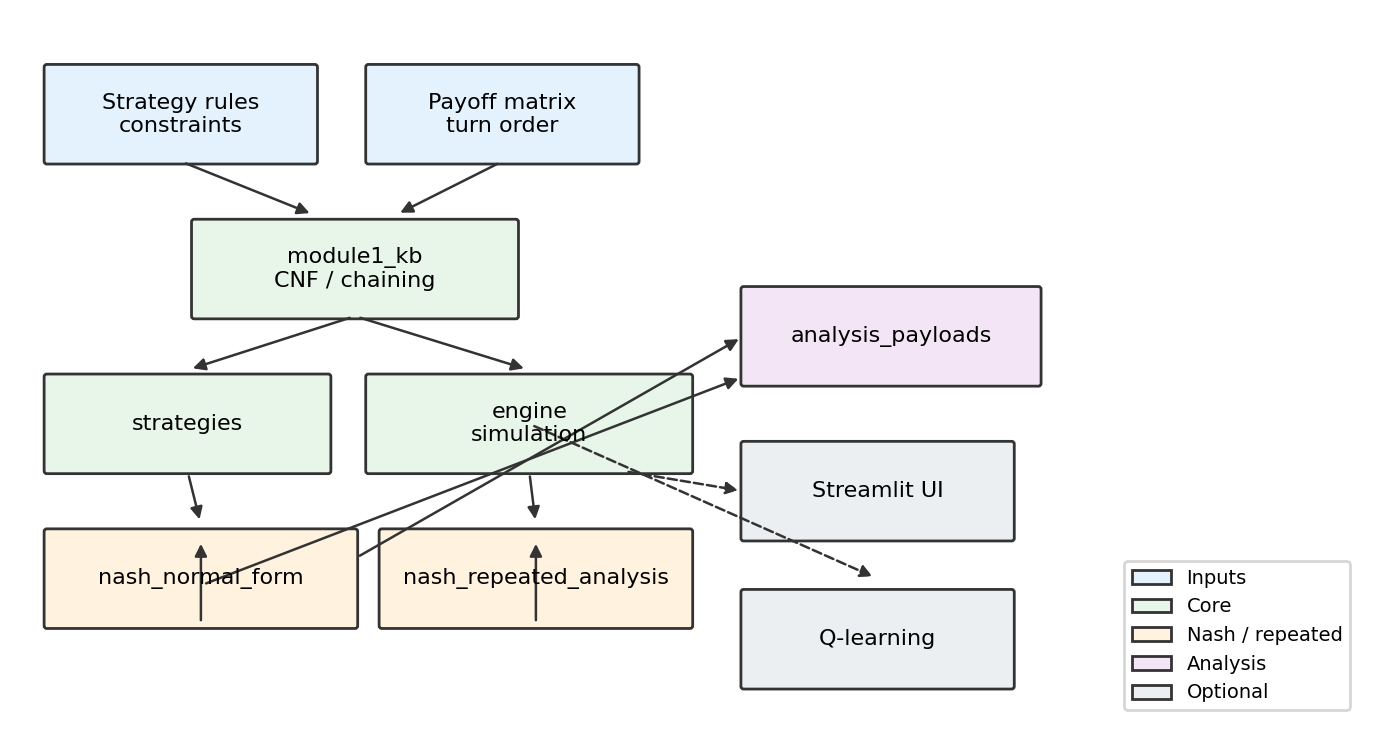
\includegraphics[width=0.95\linewidth]{figures/architecture.png}
  \caption{High-level data flow in the Chickenizer repository. Solid arrows: core library use; dashed arrows: optional UI and learning tools. Figure generated by \filepath{paper/scripts/gen_architecture_figure.py}.}
  \label{fig:arch}
\end{figure}

\textbf{Engine and strategies.} \texttt{GameEngine} holds state (actions, HP, resilience, reputation, preferences, histories, end reason). Strategies implement a shared interface in \texttt{strategies.py} and may use the knowledge base or hand-written rules. Each round updates resilience from merged preferences and checks stop rules (round cap, resilience gap, etc.). Analysis code often uses NumPy~\cite{numpy}.

\textbf{Nash (one-shot).} \filepath{nash_normal_form.py} fills a $2\times 2$ matrix by running one counterfactual round per cell from the current baseline so cells reflect resilience after that joint choice. Pure Nash is by best-response scan; mixed equilibria use Nashpy when needed. This stays separate from long multi-round runs.

\textbf{Repeated play.} \filepath{nash_repeated_analysis.py} runs many rounds with two fixed strategies and returns summaries (per-round log, action frequencies, resilience series, and averages grouped by the previous round's joint action). The code states clearly that this is not Nash equilibrium of the repeated game.

\textbf{Analysis and UI.} \filepath{analysis_payloads.py} bundles results for consumers including Streamlit under \filepath{.src/ui/}. Q-learning tournament and heatmap scripts add optional comparisons between learned policies.

\textbf{End-to-end flow.} A typical library path is: build or load strategies that respect Module~1 constraints; run the engine (Module~4) for traces; optionally call \filepath{nash_normal_form} (Module~3) on the current state to read off equilibria of the induced $2\times 2$ game; optionally call \filepath{nash_repeated_analysis} (Module~5) for long-run counts and paths; pass structured dicts or dataclasses into analysis payloads or the UI. Module~2 search logic sits inside engine/strategy calls rather than as a separate executable, but tests still treat those behaviors as part of the search story.

\textbf{Tests.} \filepath{integration_tests/} checks handoffs between modules (for example, search vs.\ Nash on small states, simulation feeding analysis). Together with Figure~\ref{fig:arch}, that gives a concrete picture of allowed dependencies.

\section{Module Implementation Summary}

Subsections follow the five-module course plan and point to real files under \texttt{.src/}. The README still mentions some \texttt{module2\_search.py}-style names that are not the main layout today.

\subsection{Module 1: Strategy Logic Encoder and Knowledge Base}
\textbf{Purpose.} Encode strategy and game rules as logic, convert to CNF, check consistency, and query consequences (forward/backward chaining).

\textbf{Inputs / outputs.} SymPy boolean formulas (implications, legal-action constraints, collision structure) in; normalized KB, satisfiability and conflicts, entailed facts out~\cite{sympy}.

\textbf{Design.} Logic lives in \texttt{module1\_kb.py} so later stages do not duplicate CNF work. Logging degrades quietly if the debug helper is missing.

\textbf{Integration.} Feeds Module~2 and strategy objects the engine runs. Without a consistent KB, downstream search and Nash code would have to re-implement rule parsing.

\subsection{Module 2: Optimal Strategy Combination Search}
\textbf{Purpose.} Search over valid moves or short horizons to favor one player under bad opponent play, matching the course search topics.

\textbf{Inputs / outputs.} Engine state, strategies, depth or similar settings in; chosen moves, traces or diagnostics, payoff-style scalars out.

\textbf{Design.} There is no single \texttt{module2\_search.py}; search- and minimax-related code sits in \texttt{engine.py}, \texttt{strategies.py}, and helpers. Behavior is covered by tests even though filenames differ from the original table.

\textbf{Integration.} \texttt{integration\_tests/module2/} ties Module~2 to Module~3 and Module~5. When search settings change, those tests are the early warning for broken cross-module numeric agreement.

\subsection{Module 3: Nash Equilibrium Solver}
\textbf{Purpose.} Nash equilibria of the induced normal form for the current state and preferences.

\textbf{Inputs / outputs.} Two strategies, baseline state, action labels in; pure (and optional mixed) profiles, payoffs, best-response summaries out~\cite{nashpy,nash1950}.

\textbf{Design.} Payoffs are resilience-based, not dollars; in-code comments explain why baseline shifts affect display but not pure Nash indices.

\textbf{Integration.} Needs Module~1 strategies and the engine for payoffs. \texttt{integration\_tests/module3/} links to downstream analysis. If engine preferences change, Nash cells and UI coloring must move together---tests anchor that coupling.

\subsection{Module 4: Chicken Game Engine and Simulation}
\textbf{Purpose.} Run sequential Chicken with alternating moves and record a full trace.

\textbf{Inputs / outputs.} Initial state, two strategies, match settings in; action history, payoffs/resilience paths, end reason out.

\textbf{Design.} One \texttt{GameEngine} implements transitions so Nash and repeated tools see the same rules.

\textbf{Integration.} Feeds Module~5; RL scripts can treat the engine as the environment. Any change to round resolution or resilience updates shows up immediately in both classroom demos and learning runs.

\subsection{Module 5: Strategy Analysis and Comparison}
\textbf{Purpose.} Combine search, Nash, and simulation outputs into tables, plots, and UI-ready data.

\textbf{Inputs / outputs.} Repeated-analysis structs, Nash results, strategy names in; tables, matplotlib-based plots~\cite{matplotlib}, Streamlit/HTML snippets where used~\cite{streamlit}.

\textbf{Design.} Prefer plain data types and functions testable without a browser.

\textbf{Integration.} \texttt{integration\_tests/module5/} covers end-to-end flows.

Table~\ref{tab:modmap} maps course module labels to primary files.

\begin{table}[t]
  \centering
  \caption{Course module labels mapped to principal files in \texttt{.src/}.}
  \label{tab:modmap}
  \begin{tabular}{@{}ll@{}}
    \toprule
    Module (course label) & Primary implementation \\
    \midrule
    1 Logic / KB & \texttt{module1\_kb.py} \\
    2 Search & \texttt{engine.py}, \texttt{strategies.py} (shared) \\
    3 Nash & \texttt{nash\_normal\_form.py} \\
    4 Simulation & \texttt{engine.py}, \texttt{match\_session.py} \\
    5 Analysis & \texttt{nash\_repeated\_analysis.py}, \texttt{analysis\_payloads.py}, UI \\
    \bottomrule
  \end{tabular}
\end{table}

\section{Evaluation Methodology}

We rely on automated regression tests, not a single leaderboard score. The repo uses \texttt{pytest} with \texttt{pytest.ini} so imports from \texttt{.src/} work under different import modes~\cite{pytest}.

\textbf{What we measure.} (1)~\textbf{Pass/fail:} full suite \texttt{pytest unit\_tests/ integration\_tests/}. (2)~\textbf{Coverage of concerns:} unit tests for KB, engine, Nash matrix code, repeated analysis, and RL smoke paths; integration tests for cross-module contracts (e.g.\ Module~2 vs.\ Module~3 on default states, Module~4 $\rightarrow$ Module~5, payload shape).

Unit tests stay close to one file or one idea so a failure names a small surface area. Integration tests are fewer on purpose: they encode agreements between teams of files (same default payoff state, same action ordering, same keys in dicts passed toward analysis). When a feature spans modules, we prefer an integration test over a giant unit test with deep mocks, because mocks can hide real import or type mistakes.

\textbf{How we collected results.} From the repo root we ran \texttt{pytest unit\_tests/ integration\_tests/ -q}: 247 collected, 247 passed, 0 failed, on the machine used while writing (about two seconds). Table~\ref{tab:pytest} splits counts by folder using \texttt{pytest --collect-only} per path. That table is the main quantitative result in this paper.

\textbf{What this does not show.} Tests only cover written scenarios; they do not prove the spec is right for every Nashpy edge case or every random RL seed. Streamlit demos and benchmark plots are supporting material, not controlled experiments. Pinning versions in \texttt{requirements.txt} limits library drift but does not remove it.

\textbf{Reproducing the numbers.} Clone the repository, install dependencies from \texttt{requirements.txt}, and run the same \texttt{pytest} command from the repository root. Counts in Table~\ref{tab:pytest} should match \texttt{pytest --collect-only} on each listed path; if they diverge after new tests are added, update the table and the prose here in the same commit so the paper stays tied to the branch you submit.

\section{Results}

\textbf{Strengths.} The full \texttt{pytest} run passed (247 tests). Most tests are unit-level, which helps catch subtle bugs in logic and resilience math; the smaller set of integration tests targets module boundaries where wiring errors usually appear.

\textbf{Weaknesses.} README filenames still diverge from the tree in places. Tests use hand-built fixtures, not external datasets. We did not run large hyperparameter sweeps or formal UI user studies.

Table~\ref{tab:pytest} lists collection counts by area; every listed test passed in the aggregate run reported above.

\begin{table}[t]
  \centering
  \caption{Tests collected by area (snapshot, April 2026). All passed in the reported full-suite run.}
  \label{tab:pytest}
  \begin{tabular}{@{}lr@{}}
    \toprule
    Area & Tests collected \\
    \midrule
    \texttt{unit\_tests/} & 239 \\
    \texttt{integration\_tests/module2/} & 2 \\
    \texttt{integration\_tests/module3/} & 1 \\
    \texttt{integration\_tests/module4/} & 1 \\
    \texttt{integration\_tests/module5/} & 2 \\
    \texttt{integration\_tests/rl/} & 2 \\
    \midrule
    Total & 247 \\
    \bottomrule
  \end{tabular}
\end{table}

Figure~\ref{fig:qlheat} shows the project's pairwise Q-learning heatmap (copied from \texttt{graphics/ql\_pairwise\_heatmap.png} into \texttt{paper/figures/} for a self-contained paper folder). It is evidence that the learning tooling produces a readable graphic, not a claim about optimal human play; axis and color meaning come from the script that generated the original asset.

If your local clone shows a different total after pulling new commits, update Table~\ref{tab:pytest} and the sentence above to match; do not keep stale counts in the PDF.

Reading Table~\ref{tab:pytest} together with the passing full-suite run supports two narrow claims: first, the low-level pieces (KB, engine, Nash helpers, repeated analysis, RL smoke) each have direct tests; second, a small but targeted set of integration tests guards the interfaces where regressions hurt most. It does \emph{not} support a claim that every feature in the Streamlit UI is exhaustively clicked in CI---only that the underlying Python contracts those screens rely on are exercised.

\begin{figure}[t]
  \centering
  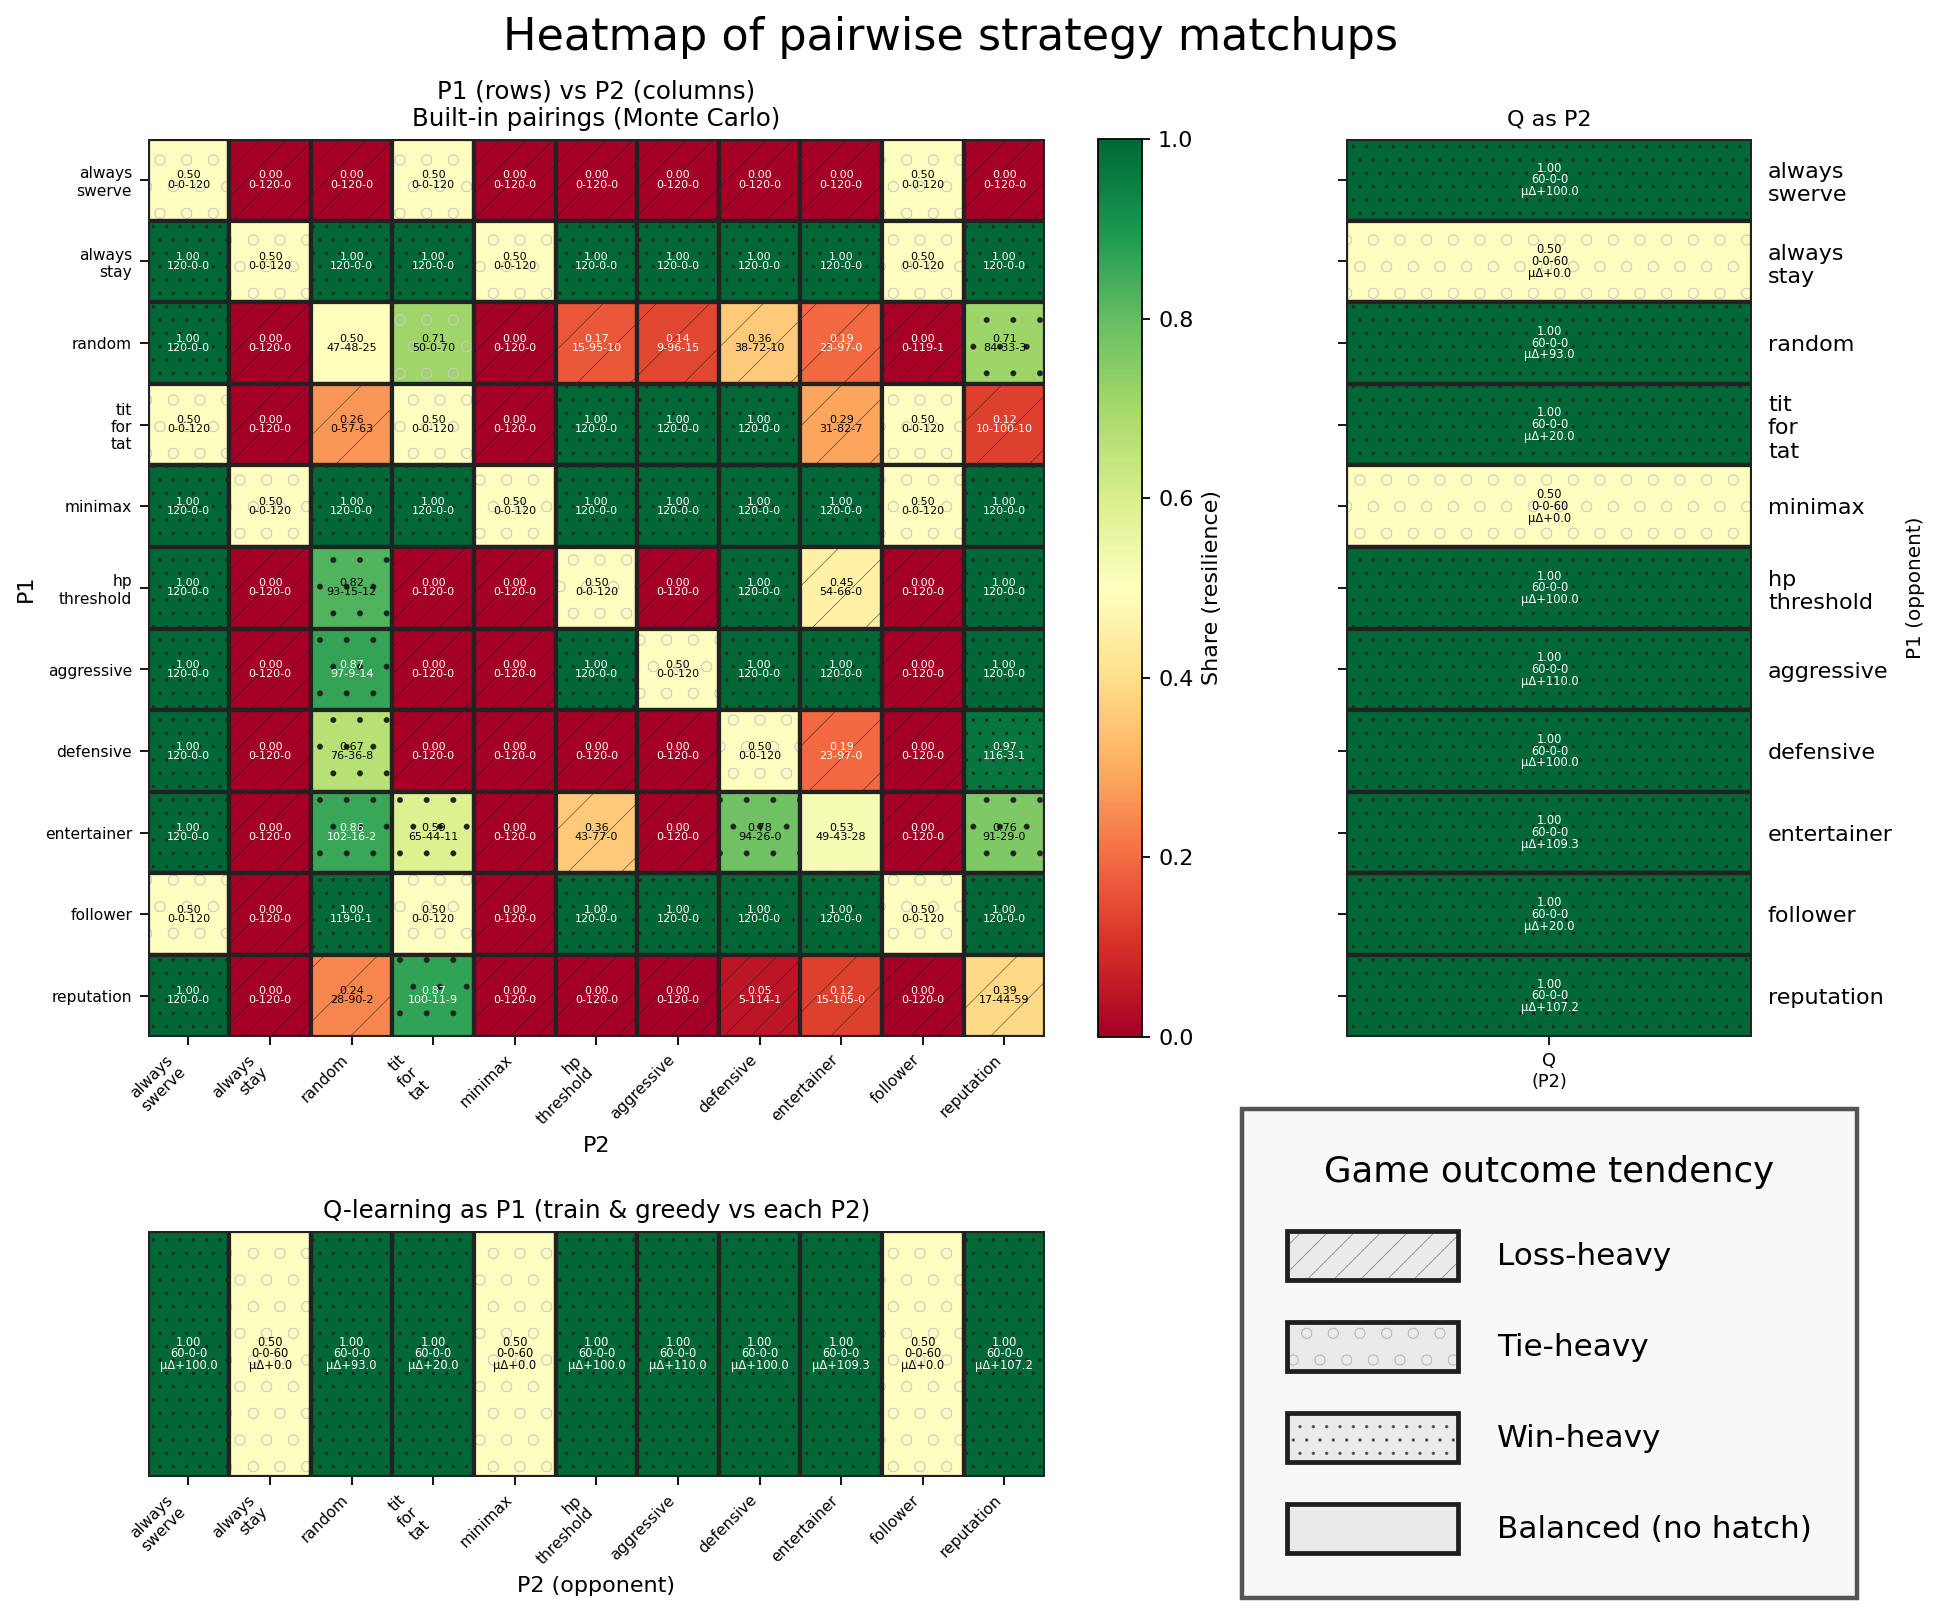
\includegraphics[width=0.72\linewidth]{figures/ql_pairwise_heatmap.png}
  \caption{Pairwise Q-learning heatmap from the project \texttt{graphics/} bundle. Read axis labels and the generator script before citing numeric cells.}
  \label{fig:qlheat}
\end{figure}

\section{Proposal Delta}

The approved proposal described five modules with names like \texttt{module2\_search.py}--\texttt{module5\_analysis.py} under a normal \texttt{src/} tree. The shipped system keeps the same five ideas but differs in packaging and extras.

\textbf{Layout.} Code runs from \texttt{.src/} (with a leading dot) and root bootstrap, not from the \texttt{src/} paths some README commands still show. Imports work when tests are configured, but copied shell commands can fail.

\textbf{Module~2.} Search and minimax-style behavior live in \texttt{engine.py} and \texttt{strategies.py} instead of one \texttt{module2\_search.py}. Tests define the boundary; filenames are the main mismatch with the proposal table.

\textbf{Streamlit UI.} The proposal discussed analysis and plots but did not require a browser app. We added Streamlit under \texttt{.src/ui/} for demos; that adds dependencies and paths to maintain.

\textbf{Q-learning add-ons.} The original five modules were classical AI topics. The repo also has Q-learning training, tournaments, traces, and \texttt{integration\_tests/rl/}. These support comparisons with hand-written strategies but are extra relative to the core Nash/simulation story.

\textbf{Repeated-game wording.} The proposal can read as promising full repeated-game Nash theory. \texttt{nash\_repeated\_analysis.py} instead implements simulated summaries over many rounds and states that in the file header---a smaller, testable scope.

\textbf{Why change.} Shared engine code avoids two different ``physics'' for Nash vs.\ simulation; the UI helps classroom demos; repeated analysis stays honest about what it is. A thin \texttt{module2\_search.py} wrapper could reduce README drift later without changing behavior.

\textbf{What we did not drop.} All five course topics still appear in running code and tests: logic in \texttt{module1\_kb.py}, search behavior in engine/strategies, Nash in \texttt{nash\_normal\_form.py}, simulation in the engine and session helpers, and analysis in repeated-analysis and payload modules plus UI. Optional RL files add scope rather than replacing those five roles.

\section{Limitations and Failure Analysis}

\textbf{1. README vs.\ runnable tree.} The README still points at some \filepath{src/...} commands that do not match today's files, while developers use \filepath{.src/} and \filepath{python -m pytest}. Likely causes: refactors ahead of docs, and an unusual dotted folder name. \textbf{Effect:} wasted setup time or false ``project broken'' reports. \textbf{Mitigation:} add thin wrapper scripts at the documented paths, or rewrite README commands and CI-check them.

\textbf{2. Nash layer is partial.} One-shot Nash uses a $2\times 2$ matrix from counterfactual resilience after one joint move from the current state. That can miss incentives that only show up over many rounds. Mixed Nash depends on Nashpy numerics we do not fully stress-test. \textbf{Failure mode:} readers treat UI colors as subgame-perfect advice. \textbf{Mitigation:} clearer UI labels, more integration tests on long-run action frequencies vs.\ static Nash where both are defined.

\textbf{3. Tests vs.\ hostile code.} 247 passing tests still assume well-behaved strategies and fixtures. Malicious or sloppy code could mutate globals or skip the KB. \textbf{Mitigation:} stricter interfaces, property tests on small strategy algebras, light fuzzing on payoff inputs within bounds.

Separately, any paper can lag the branch: if you merge new features after drafting, rerun \filepath{python -m pytest unit_tests integration_tests -q} and refresh counts before PDF export. The course expects you to report what actually ran, not what you plan to run later.

\section{Individual Contributions}

Effort shares below use \textbf{commit counts} on this repository as a starting point (Greyson as \texttt{cptareb}: 55 commits; Will as \texttt{William Zoeller}: 34; classroom bot excluded). That ratio is $55{:}34 \approx 62\%{:}38\%$. \textit{Adjust the percentages and bullets if your real split differs}---the course cares about honest effort, not git noise.

\textbf{Greyson Henry (62\%):}
\begin{itemize}
  \item Heavy development on the knowledge base (\texttt{module1\_kb.py}), strategies (\texttt{strategies.py}), engine (\texttt{engine.py}), Nash normal form (\texttt{nash\_normal\_form.py}), and Q-learning training (\texttt{train\_ql.py}), with matching unit tests.
  \item Streamlit features and panels (including \texttt{streamlit\_app.py} and hypothesis-related UI), co-evolving with Will's UI work.
  \item Broad unit test coverage for engine, strategies, Nash, and Q-learning paths.
\end{itemize}

\textbf{Will Zoeller (38\%):}
\begin{itemize}
  \item Frequent commits to the Streamlit entry point (\texttt{streamlit\_app.py}) and integration tests under \texttt{integration\_tests/module4/}, \texttt{module5/}, and \texttt{rl/}.
  \item Checkpoint and rubric reports under \texttt{rubrics/}, plus shared edits to \texttt{module1\_kb.py}, \texttt{strategies.py}, Nash/repeated-analysis tests, and README.
  \item Connected simulation and analysis outputs to UI panels used in demos.
\end{itemize}

\textbf{Paper for CSC 343:} Both members reviewed the codebase for accuracy; Greyson prepared the LaTeX draft under \texttt{paper/} with Will's spot-check on technical claims.

\section{Conclusions and Future Work}

Chickenizer ties together a SymPy knowledge base~\cite{sympy}, a shared simulation engine, one-shot Nash analysis via Nashpy~\cite{nashpy,nash1950}, repeated-match summaries, analysis payloads, optional Streamlit~\cite{streamlit}, and small Q-learning benchmarks. On the evaluated snapshot, \texttt{pytest} reports 247 passing tests across unit and integration suites~\cite{pytest}.

The best structural choice is one engine for both equilibrium and simulation tools, so comparisons stay apples-to-apples. The largest practical gap is documentation drift vs.\ real paths.

\textbf{Next steps (rough priority).} (1)~Fix README/\texttt{.src/} mismatch (wrappers or doc-only rewrites with CI). (2)~If desired, add optional finite-horizon subgame-perfect tooling, clearly separate from the current induced matrix. (3)~For RL claims, log seeds and save CSVs from repeated runs. (4)~Short Streamlit usability pass if time. (5)~Automate a check that every README command exists.

For a course setting, the durable artifact is not the PDF alone but the combination of runnable code, pinned libraries, and tests that a future reader can execute. Keeping those three aligned is the simplest way to stay inside the integrity rules while still telling an interesting story about Chicken.


\bibliographystyle{unsrtnat}
\bibliography{refs}

\end{document}
